\documentclass[11pt,a4paper]{article}

\usepackage[utf8]{inputenc}
\usepackage[T1]{fontenc}
\usepackage[english]{babel}
\usepackage[a4paper,margin=2.1cm]{geometry}
\usepackage{microtype}
\usepackage{xcolor}
\usepackage{hyperref}
\usepackage{enumitem}
\usepackage{listings}
\usepackage{graphicx}
\usepackage{tikz}
\usepackage{float}

\usetikzlibrary{arrows.meta,positioning,calc,fit,shapes.geometric}

\definecolor{projectblue}{HTML}{1F4E79}
\definecolor{projectgreen}{HTML}{2F7D57}
\definecolor{projectorange}{HTML}{C26A2E}
\definecolor{projectgray}{HTML}{F3F5F7}
\definecolor{codegray}{HTML}{F7F7F7}
\definecolor{textgray}{HTML}{444444}

\hypersetup{
  colorlinks=true,
  linkcolor=projectblue,
  urlcolor=projectblue
}

\lstdefinestyle{terminal}{
  basicstyle=\ttfamily\small,
  backgroundcolor=\color{codegray},
  frame=single,
  framerule=0.2pt,
  rulecolor=\color{projectblue!35},
  breaklines=true,
  columns=fullflexible,
  keepspaces=true,
  showstringspaces=false
}

\setlist[itemize]{leftmargin=1.35em,itemsep=0.25em,topsep=0.35em}
\setlist[enumerate]{leftmargin=1.5em,itemsep=0.25em,topsep=0.35em}

\newcommand{\diagramcaption}[1]{%
  \par\vspace{0.35em}
  {\small\itshape #1}
  \par\vspace{0.8em}
}

\title{\textbf{Project Demo Notes}\\
\large eBPF security monitoring tool\\[0.5em]
\normalsize Politecnico di Torino\\
\normalsize Rakuten Mobile}
\author{Simone Romano \ Giuseppe Insalaco}
\date{May 2026}

\begin{document}

\maketitle

\section*{Introduction}

This document is meant as a lightweight support for the first technical demo.
Rather than presenting the whole project from scratch, it focuses on the
current state of the prototype: what is already working, how the runtime path is
organized, and which parts are useful to observe during the live execution.

\section{Goal}

This demo shows the current end-to-end pipeline:

\begin{itemize}
  \item selected kernel hooks are attached from Go;
  \item events are sent through ring buffer or perf buffer;
  \item userspace decodes raw bytes into structured events;
  \item filters reduce noise;
  \item output is printed as \texttt{table} or \texttt{json}.
\end{itemize}

This is not yet a detection engine. The goal of the demo is to show that the
event collection pipeline works and that the architecture is ready for
enrichment and detection logic.

\section{Current Pipeline}

\begin{center}
\resizebox{0.98\textwidth}{!}{%
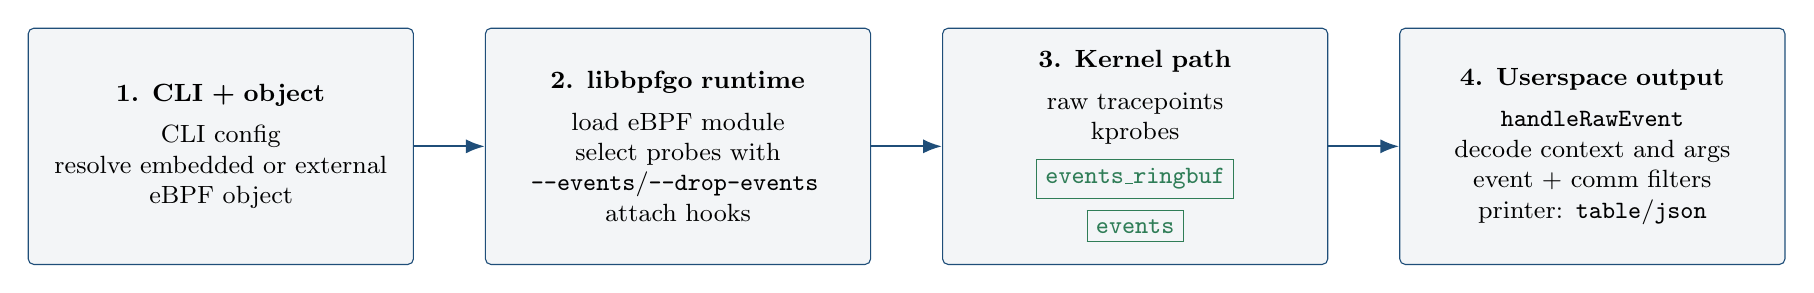
\begin{tikzpicture}[
  node distance=0.75cm,
  stage/.style={
    rectangle,
    rounded corners=2pt,
    draw=projectblue,
    fill=projectgray,
    text width=4.4cm,
    align=center,
    minimum height=3.0cm,
    inner sep=7pt,
    font=\small
  },
  transport/.style={
    rectangle,
    rounded corners=2pt,
    draw=projectgreen,
    fill=projectgreen!8,
    text width=3.9cm,
    align=center,
    minimum height=0.62cm,
    font=\footnotesize
  },
  arrow/.style={-{Latex[length=2.4mm]}, thick, draw=projectblue}
]

\node[stage] (cli) at (0,0) {
  \textbf{1. CLI + object}\\[4pt]
  CLI config\\
  resolve embedded or external\\
  eBPF object
};

\node[stage, right=0.9cm of cli] (runtime) {
  \textbf{2. libbpfgo runtime}\\[4pt]
  load eBPF module\\
  select probes with\\
  \texttt{--events}/\texttt{--drop-events}\\
  attach hooks
};

\node[stage, right=0.9cm of runtime] (kernel) {
  \textbf{3. Kernel path}\\[4pt]
  raw tracepoints\\
  kprobes\\[5pt]
  {\color{projectgreen}\fbox{\texttt{events\_ringbuf}}}\\[3pt]
  {\color{projectgreen}\fbox{\texttt{events}}}
};

\node[stage, right=0.9cm of kernel] (user) {
  \textbf{4. Userspace output}\\[4pt]
  \texttt{handleRawEvent}\\
  decode context and args\\
  event + comm filters\\
  printer: \texttt{table}/\texttt{json}
};

\draw[arrow] (cli) -- (runtime);
\draw[arrow] (runtime) -- (kernel);
\draw[arrow] (kernel) -- (user);

\end{tikzpicture}}
\diagramcaption{Figure 1: Current execution pipeline of the tool.}
\end{center}

\section{What Works Today}

\begin{itemize}
  \item eBPF object build through \texttt{make bpf}.
  \item Go userspace runtime based on \texttt{libbpfgo}.
  \item Probe registry in \texttt{pkg/ebpf/probes}.
  \item Event selection with \texttt{--events} and \texttt{--drop-events}.
  \item Command-name filtering with \texttt{--comms}.
  \item Ring buffer reader for process/security events.
  \item Perf buffer reader for Tracee-like/networking events.
  \item Output layer with \texttt{json} and \texttt{table}.
\end{itemize}

\section{Event Groups}

\begin{center}
\resizebox{0.96\textwidth}{!}{%
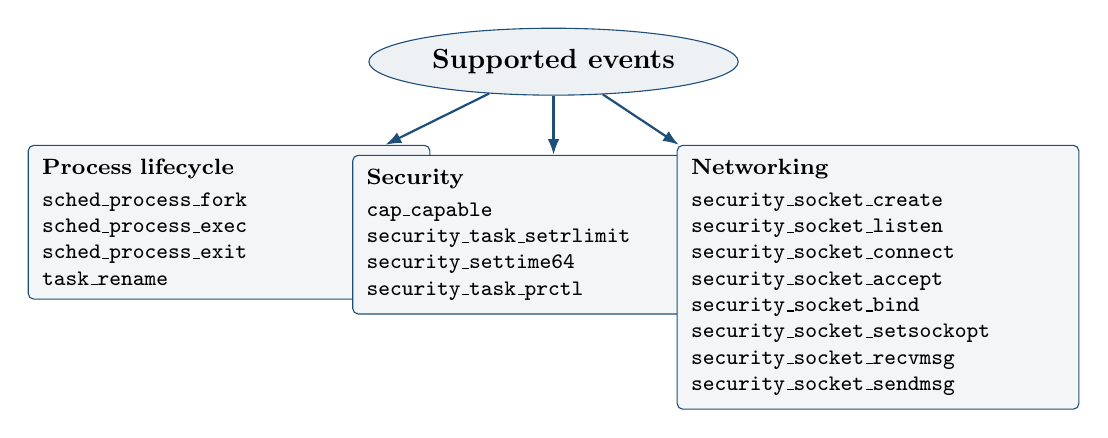
\begin{tikzpicture}[
  root/.style={
    ellipse,
    draw=projectblue,
    fill=projectblue!8,
    minimum width=4.0cm,
    minimum height=0.85cm,
    align=center,
    font=\bfseries
  },
  group/.style={
    rectangle,
    rounded corners=2pt,
    draw=projectblue,
    fill=projectgray,
    text width=4.75cm,
    align=left,
    inner sep=5pt,
    font=\footnotesize
  },
  arrow/.style={-{Latex[length=2mm]}, thick, draw=projectblue}
]

\node[root] (root) {Supported events};

\node[group, below left=0.75cm and -0.1cm of root] (process) {
  \textbf{Process lifecycle}\\[2pt]
  \texttt{sched\_process\_fork}\\
  \texttt{sched\_process\_exec}\\
  \texttt{sched\_process\_exit}\\
  \texttt{task\_rename}
};

\node[group, below=0.75cm of root] (security) {
  \textbf{Security}\\[2pt]
  \texttt{cap\_capable}\\
  \texttt{security\_task\_setrlimit}\\
  \texttt{security\_settime64}\\
  \texttt{security\_task\_prctl}
};

\node[group, below right=0.75cm and -0.1cm of root] (network) {
  \textbf{Networking}\\[2pt]
  \texttt{security\_socket\_create}\\
  \texttt{security\_socket\_listen}\\
  \texttt{security\_socket\_connect}\\
  \texttt{security\_socket\_accept}\\
  \texttt{security\_socket\_bind}\\
  \texttt{security\_socket\_setsockopt}\\
  \texttt{security\_socket\_recvmsg}\\
  \texttt{security\_socket\_sendmsg}
};

\draw[arrow] (root) -- (process);
\draw[arrow] (root) -- (security);
\draw[arrow] (root) -- (network);

\end{tikzpicture}}
\diagramcaption{Figure 2: Supported event families.}
\end{center}

\section{Demo Flow}

\subsection{1. Build the Tool}

\begin{lstlisting}[style=terminal]
cd demo_project
make build
\end{lstlisting}

Expected result:

\begin{lstlisting}[style=terminal]
dist/project.bpf.o
dist/project
\end{lstlisting}

\subsection{2. Show Process Execution Events}

Terminal 1:

\begin{lstlisting}[style=terminal]
sudo ./dist/project \
  --events task_rename,sched_process_exec,sched_process_exit \
  --comms ls,whoami \
  --output table
\end{lstlisting}

Terminal 2:

\begin{lstlisting}[style=terminal]
ls
whoami
\end{lstlisting}

Expected output shape:

\begin{lstlisting}[style=terminal]
event=task_rename pid=... tid=... uid=1000 comm=bash args=old_name=bash,new_name=ls
event=sched_process_exec pid=... tid=... uid=1000 comm=ls args=filename=/usr/bin/ls
event=sched_process_exit pid=... tid=... uid=1000 comm=ls args=exit_code=0,group_dead=1
\end{lstlisting}

What to explain:

\begin{itemize}
  \item \texttt{task\_rename} shows the task \texttt{comm} transition.
  \item \texttt{sched\_process\_exec} shows the executed binary path.
  \item \texttt{sched\_process\_exit} shows process termination and exit code.
  \item \texttt{--comms} keeps the output focused on the commands used in the demo.
\end{itemize}

\subsection{3. Show Networking Event Path}

Terminal 1:

\begin{lstlisting}[style=terminal]
make filtered
\end{lstlisting}

Terminal 2:

\begin{lstlisting}[style=terminal]
python3 -m http.server 18080 --bind 127.0.0.1
\end{lstlisting}

Terminal 3:

\begin{lstlisting}[style=terminal]
curl http://127.0.0.1:18080
\end{lstlisting}

What to explain:

\begin{itemize}
  \item \texttt{security\_socket\_connect} is attached as a kprobe.
  \item Networking hooks currently follow the perf-buffer path.
  \item The runtime now reads both ring buffer and perf buffer.
\end{itemize}

\subsection{4. Optional: Show a Sensitive Security Hook}

Terminal 1:

\begin{lstlisting}[style=terminal]
sudo ./dist/project --events security_settime64 --output table
\end{lstlisting}

Terminal 2:

\begin{lstlisting}[style=terminal]
sudo date -s "$(date '+%Y-%m-%d %H:%M:%S')"
\end{lstlisting}

What to explain:

\begin{itemize}
  \item \texttt{security\_settime64} is triggered when a process tries to modify system time.
  \item It requires privileges such as \texttt{CAP\_SYS\_TIME}.
  \item Use this only on a test VM.
\end{itemize}

\section{Architecture Talking Points}

\begin{center}
\resizebox{0.98\textwidth}{!}{%
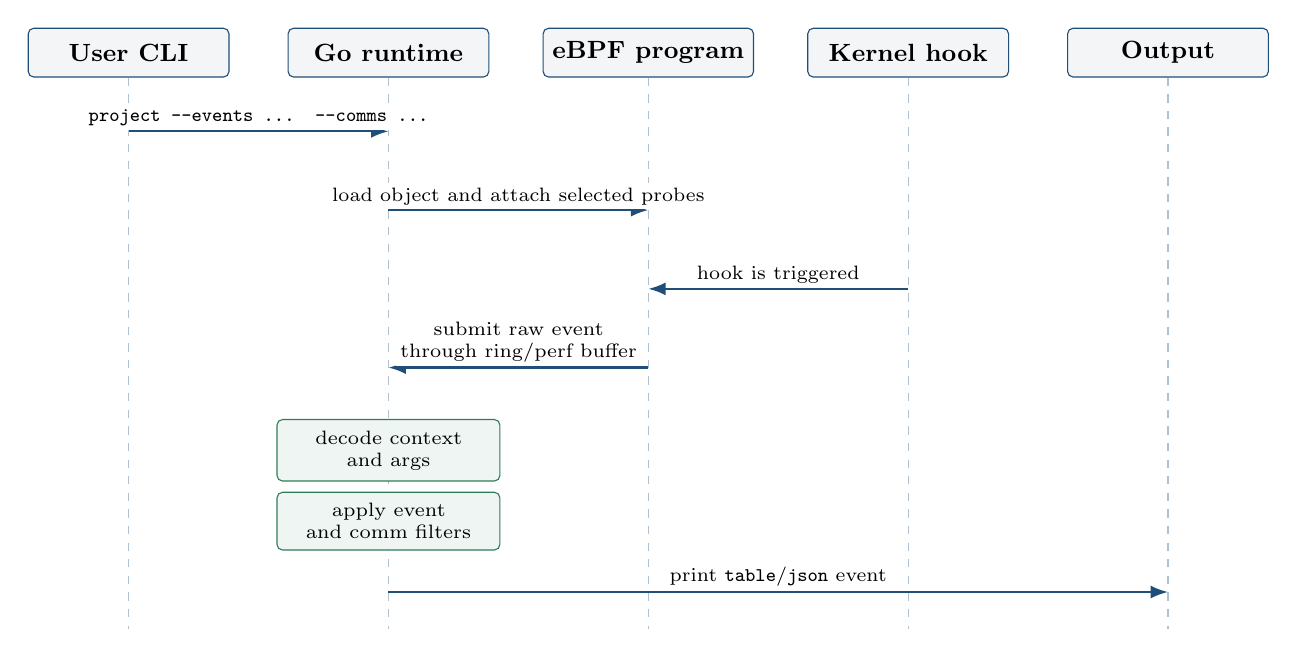
\begin{tikzpicture}[
  participant/.style={
    rectangle,
    rounded corners=2pt,
    draw=projectblue,
    fill=projectgray,
    minimum width=2.55cm,
    minimum height=0.62cm,
    align=center,
    font=\small\bfseries
  },
  lifeline/.style={draw=projectblue!35, dashed},
  msg/.style={-{Latex[length=2.2mm]}, thick, draw=projectblue},
  label/.style={
    font=\scriptsize,
    align=center,
    fill=white,
    inner sep=1.5pt,
    text=black
  },
  action/.style={
    rectangle,
    rounded corners=2pt,
    draw=projectgreen,
    fill=projectgreen!8,
    text width=2.55cm,
    align=center,
    inner sep=4pt,
    font=\scriptsize
  }
]

\node[participant] (user) at (0,0) {User CLI};
\node[participant] (go) at (3.3,0) {Go runtime};
\node[participant] (bpf) at (6.6,0) {eBPF program};
\node[participant] (kernel) at (9.9,0) {Kernel hook};
\node[participant] (out) at (13.2,0) {Output};

\foreach \p in {user,go,bpf,kernel,out} {
  \draw[lifeline] (\p.south) -- ++(0,-7.0);
}

\draw[msg] ($(user)+(0,-1.0)$) --
  node[label, above] {\texttt{project --events ... --comms ...}}
  ($(go)+(0,-1.0)$);

\draw[msg] ($(go)+(0,-2.0)$) --
  node[label, above] {load object and attach selected probes}
  ($(bpf)+(0,-2.0)$);

\draw[msg] ($(kernel)+(0,-3.0)$) --
  node[label, above] {hook is triggered}
  ($(bpf)+(0,-3.0)$);

\draw[msg] ($(bpf)+(0,-4.0)$) --
  node[label, above, text width=3.0cm] {submit raw event through ring/perf buffer}
  ($(go)+(0,-4.0)$);

\node[action] (decode) at ($(go)+(0,-5.05)$) {decode context\\and args};
\node[action] (filters) at ($(go)+(0,-5.95)$) {apply event\\and comm filters};

\draw[msg] ($(go)+(0,-6.85)$) --
  node[label, above] {print \texttt{table}/\texttt{json} event}
  ($(out)+(0,-6.85)$);

\end{tikzpicture}}
\diagramcaption{Figure 3: High-level interaction between CLI, Go runtime, eBPF code, kernel hooks and output.}
\end{center}

Key points:

\begin{itemize}
  \item The tool does not attach every probe blindly when \texttt{--events} is used.
  \item The decoder is intentionally separated from output formatting.
  \item The output layer can evolve without changing the eBPF runtime.
  \item The current design is close to Tracee conceptually, but smaller and easier to reason about for the thesis.
\end{itemize}

\section{Known Limits}

\begin{itemize}
  \item Some arguments are still raw numeric values.
  \item \texttt{security\_task\_prctl} needs symbolic mapping for options like \texttt{PR\_SET\_VMA}.
  \item Socket addresses and socket constants need better human-readable formatting.
  \item \texttt{--comms} is a userspace filter, so it improves output readability but does not reduce kernel-side work.
  \item The final transport strategy still needs consolidation: keep both ring/perf buffers, or converge to perf buffer in a more Tracee-like design.
  \item Detection logic and MITRE ATT\&CK mapping are future work.
\end{itemize}

\section{Short Closing}

The current version demonstrates the hard part of the project: a working
kernel-to-userspace event pipeline on the target Rocky Linux kernel. The next
step is not loading eBPF anymore, but improving event semantics: better
argument mapping, stronger filters and eventually detection logic.

\end{document}
